% This file was converted to LaTeX by Writer2LaTeX ver. 0.4
% see http://www.hj-gym.dk/~hj/writer2latex for more info
\documentclass[11pt,twoside]{article}
\usepackage{graphicx}
\usepackage[ascii]{inputenc}
\usepackage[T1]{fontenc}
\usepackage{amsmath,amssymb,amsfonts,textcomp}
\usepackage{color}
\usepackage{alltt}
\usepackage{calc}
\usepackage{hyperref}
\hypersetup{colorlinks=true, linkcolor=blue, filecolor=blue, pagecolor=blue, urlcolor=blue}

%% Define a new 'url' style for the url package that will use a smaller font.
\makeatletter
\def\url@urlstyle{%
  \@ifundefined{selectfont}{\def\UrlFont{\sf}}{\def\UrlFont{\small\ttfamily}}}
\makeatother
%% Now actually use the newly defined style.
\urlstyle{urlstyle}

% Pages styles (master pages)
\setlength\parindent{0in}
\setlength{\parskip}{1ex plus 0.5ex minus 0.2ex}
\setlength\textwidth{6.5in}
\makeatletter
\newcommand\ps@Standard{%
\renewcommand\@oddhead{}%
\renewcommand\@evenhead{\@oddhead}%
\renewcommand\@oddfoot{}%
\renewcommand\@evenfoot{\@oddfoot}%
\setlength\paperwidth{8.5in}\setlength\paperheight{11in}\setlength\voffset{-1in}\setlength\hoffset{-1in}\setlength\topmargin{0.5in}\setlength\headheight{12pt}\setlength\headsep{0.461in}\setlength\footskip{12pt+0.461in}\setlength\textheight{11in-0.5in-0.5in-0.461in-12pt-0.461in-12pt}\setlength\oddsidemargin{1in}\setlength\textwidth{8.5in-1in-1in}
\renewcommand\thepage{\arabic{page}}
\setlength{\skip\footins}{0.0398in}\renewcommand\footnoterule{\vspace*{-0.0071in}\noindent{\rule{0.25\columnwidth}{0.0071in}}\vspace*{0.0398in}}
}
\makeatother
\pagestyle{Standard}
% footnotes configuration
\makeatletter
\renewcommand\thefootnote{\arabic{footnote}}
\makeatother

\newcommand{\cmd}[1]
   {\mbox{\sf #1}\null}
\newcommand{\code}[1]
   {\mbox{\bf\tt #1}\null}
\newcommand{\file}[1]
   {\mbox{\bf\em #1}\null}
\newcommand{\param}[1]
   {\mbox{\{\em #1\}}\null}
\newenvironment{source}
{\small\begin{quote}\begin{alltt}}
{\end{alltt}\end{quote}\normalsize}

\title{Sierra IO System}
\begin{document}
\clearpage\pagestyle{Standard}
\title{Sierra IO System}
\author{Gregory D. Sjaardema\\
	Advanced Computational Mechanics Architectures\\
	Sandia-2017 National Laboratories}

\maketitle

\setcounter{tocdepth}{3}
\setlength{\parskip}{0ex plus 0.5ex minus 0.2ex}
\tableofcontents

\section{Introduction}
The documentation below is a medium{}- to low{}-level view of the Sierra
IO system targeted at developers who will be adding or modifying the
database IO portion of the system. It should give enough detail that a
new database type could be added by reading this document and looking
at an existing database class. It is also helpful to have the
doxygen{}-generated documentation for the Ioss class hierarchy
available.

The IO Subsystem has been designed to support multiple database formats
simultaneously. It is possible to have the finite element model read
from an ExodusII database; two results files being written to an
ExodusII file with a third results file being written to a CGNS file;
and the restart file being written to yet another ExodusII file. Each of
these output databases can have a different schedule for when to write
and what data is to be written.

If there are any questions or corrections, please contact Greg Sjaardema
at (505) 844{}-2701 or \href{mailto:gdsjaar@sandia.gov}{\nolinkurl{gdsjaar@sandia.gov}}.

\setlength{\parskip}{1ex plus 0.5ex minus 0.2ex}
\section{Class Structure Overview}
The three main modules or namespaces involved in the IO are:
\begin{description}
\item [\code{Fmwk}] Main sierra framework namespace. This
defines and manages the Sierra applications data structures,
algorithms, mechanics, etc. Each \code{Fmwk::Region} owns a
\code{Frio::IOBroker} which is its link to all bulk data io.
\item [\code{Frio}] The bridge between the Sierra frameworks
data structures and the IO databases data structures in the Ioss
namespace. Ideally all data transfers between Sierra and the IO
databases is under the control of the \code{Frio} classes.
However, there are some special cases where an application will
directly interact with the Ioss classes. The
\code{Frio::IOBroker} manages the Restart, Mesh, Results, and
other databases used by a \code{Fmwk::Region.}
\item [\code{Ioss}] The \code{Ioss} namespace
contains several classes which attempt to provide an abstract interface
to multiple concrete database types. It also defines a lightweight
generic representation of the finite element model.
\end{description}

\subsection{The Ioss Module}
There are two major pieces of the \code{Ioss} module: The
\code{Ioss::DatabaseIO} which is a pure virtual base class
from which all concrete IO databases are derived and the
\code{Ioss::GroupingEntity} classes which define a
lightweight generic model representation.

The current inheritance structure of
\code{Ioss::DatabaseIO} is shown in Figure~\ref{fig:dbio_inherit}.
\begin{figure}[htp]
\centering
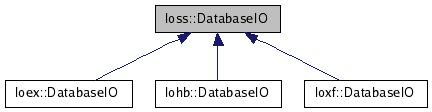
\includegraphics[scale=0.75]{DatabaseIO__inherit__graph.png}
\caption{\code{Ioss::DatabaseIO} Inheritance Diagram}\label{fig:dbio_inherit}
\end{figure}
Currently the concrete database types are ExodusII (\code{Ioex}), CGNS
(\code{Iocgns}), and Heartbeat (\code{Iohb}). The
\code{Ioss::DatabaseIO} class has a pointer to an \code{Ioss::Region
}which is the root of the generic model representation.

\subsubsection{Ioss::Region and Ioss::GroupingEntity Classes}
An \code{Ioss::Region} is an
\code{Ioss:GroupingEntity} and it contains a vector of
\code{NodeBlocks}, \code{ElementBlocks},
\code{SideSets}, and \code{CommSets} defining the current model. These are all
also \code{Ioss::GroupingEntities}. The
\code{Ioss::GroupingEntity} inheritance structure is shown in Figure~\ref{fig:ge_inherit}.
\begin{figure}[htp]
\centering
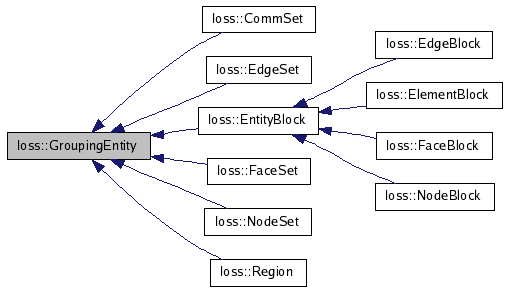
\includegraphics[scale=0.75]{GroupingEntity__inherit__graph.png}
\caption{\code{Ioss::GroupingEntity} Inheritance Diagram}\label{fig:ge_inherit}
\end{figure}
An \code{Ioss::GroupingEntity}
contains an \code{Ioss::PropertyManager} which maintains 1 or
more \code{Ioss::Property;} and an
\code{Ioss::FieldManager} which maintains 1 or
more\code{ Ioss::Field}. It also contains a name and a
pointer to the \code{Ioss::DatabaseIO}. There is also an
\code{Ioss::EntityBlock} which contains 1 extra member which
is the \code{Ioel::ElementTopology} which is the topology of
the entities contained in this block. The collaboration diagram for
the \code{Ioss::GroupingEntity} is shown in Figure~\ref{fig:ge_collab}
\begin{figure}[htp]
\centering
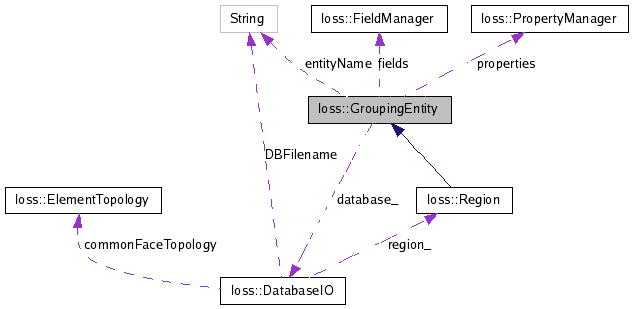
\includegraphics[scale=0.75]{GroupingEntity__coll__graph.png}
\caption{\code{Ioss::GroupingEntity} Collaboration Diagram}\label{fig:ge_collab}
\end{figure}

A \code{GroupingEntity} is a very lightweight class; it does
not contain any bulk data. It represents a portion of the finite
element model and can transfer bulk data to/from the database from/to
the Sierra datastructures. It also contains metadata about that portion
of the finite element model. Each specific
\code{GroupingEntity} type has a few required properties and
fields and some optional properties and fields. 

The \code{Ioss::GroupingEntity}'s define the basic finite
element model. For example, a model with two element blocks, a nodeset,
and two sidesets is shown in Figure~\ref{fig:block}.
\begin{figure}[htp]
\centering
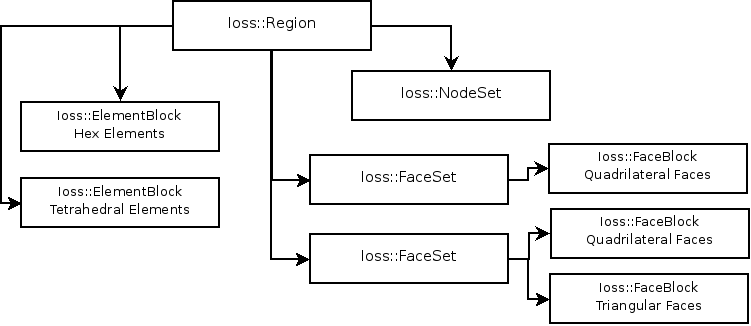
\includegraphics[scale=0.5]{Block_Diagram_Model.png}
\caption{Block Diagram of Finite Element Model Structure}\label{fig:block}
\end{figure}

Note that the \code{SideSets} are further divided into one or more
\code{SideBlocks} which contain entities of homogenous topology.

Each of these \code{GroupingEntity's} contain both
\code{Properties} and \code{Field} definitions
which can be queried by the \code{Frio} classes to define the
model.

\subsubsection{Ioss::Property and Ioss::PropertyManager}
Each \code{Ioss::GroupingEntity} class contains an
\code{Ioss::PropertyManager} which manages the
\code{Ioss::Property} on this particular entity. An
\code{Ioss::Property} is basically a named integer, real,
string, or pointer value. The \code{PropertyManager}
maintains a list of all \code{Properties} for a specific
entity and provides an interface where the \code{Properties}
can be located by name.

\subsubsection{Ioss::Field and Ioss::FieldManager}
Each \code{Ioss::GroupingEntity} class contains an
\code{Ioss::FieldManager} which manages the
\code{Ioss::Field}s on this particular entity. An
\code{Ioss::Field} contains the metadata for the field it
describes; it does not hold the bulk data, so an
\code{Ioss::Field} is fairly lightweight. Each
\code{Ioss::Field} contains:

\begin{itemize}
\item {
std::string \code{name} -- The name of the field.}
\item {
Int \code{rawCount\_} -- The size of the untransformed
field }
\item {
Int \code{transCount\_} -- The size of the transformed
field.}
\item {
BasicType \code{type\_} -- The basic type of the field
(Integer, Real, String)}
\item {
const VariableType * \code{rawStorage\_} -- The storage
type of the untransformed field (Vector, Scalar, Tensor, ....)}
\item {
const VariableType * \code{transStorage\_} -- The storage
type of the transformed field (Vector, Scalar, Tensor, ...)}
\item {
RoleType \code{role\_} -- The ``role'' of the field. Valid
roles are: \code{INTERNAL}, \code{MESH}, \code{ATTRIBUTE},
\code{COMMUNICATION}, \code{INFORMATION},
\code{REDUCTION}, and \code{TRANSIENT}. The most
common are \code{MESH} for describing the model
geometry/topology, \code{ATTRIBUTE} for block entity attributes
(typically \code{ElementBlock} at this time), \code{TRANSIENT} for time{}-dependent
results data, and \code{REDUCTION} for ``summary fields''
(see below).}
\item {
Int \code{size\_} -- The number of bytes required to store
the entire \code{Field}. Equal to \code{rawCount\_
* sizeof(type\_) * (rawStorage\_ components)}. }
\item {
std::vector{\textless} Iotr::Transform * {\textgreater} 
\code{ransforms\_} -- A list of transforms which are
applied to this field. \textit{Note that the transforms are implemented
at the Field level, but are not yet functional in Sierra
applications.}}
\end{itemize}
The \code{Ioss::Fields} are used for all bulk data input and
output. Each \code{Ioss::GroupingEntity }contains a
\code{get\_field\_data} and a
\code{put\_field\_data} function. The function signatures
are:
\begin{source}
int get\_field\_data(const std::string \&field\_name, void *data, size\_t data\_size=0)
int put\_field\_data(const std::string \&field\_name, void *data, size\_t data\_size=0)
\end{source}

The functions will get or put the data corresponding to the field
named \code{field\_name}; the data will be read from/written to the
memory pointed to by \code{data} which is of size \code{data\_size}.
If \code{data\_size} is nonzero, then the field checks that there is
sufficient space to store the field data; if it is zero, then it is
assumed to be large enough.  The function returns the number of
entities for which the field was read/written.

The \code{get\_field\_data} and
\code{put\_field\_data} functions are actually at
the\code{ Ioss::GroupingEntity} level and they forward the
call down to \code{internal\_get\_field\_data} and
\code{internal\_put\_field\_data} which are defined on each
class derived from \code{Ioss::GroupingEntity.} These in turn
call\footnote{The \code{offset} and \code{count}
were originally intended to provide partial field input and output, but
this became too unwieldy and is not used at this time. Only full field
input or output is supported.}:
\begin{source}
int get\_database(){}-{\textgreater}get\_field(this, field, offset, count, data, data\_size);
\end{source}

get the concrete database class which is responsible for transferring
the bulk data to/from the database to/from the memory pointed to by
\code{data} of size \code{data\_size} bytes.

\paragraph{Ioss::Field -- Roles}
As defined above, there are six values for a fields
\code{role}. The three most commonly used are:

\begin{description}
\item [\code{MESH}] A field which is used to define the basic
geometry or topology of the model and is not normally transient in
nature. Examples would be element connectivity or nodal coordinates.
\item [\code{ATTRIBUTE}] A field which is used to define an attribute
on an \code{EntityBlock} derived class.  Examples would be thickness
of the elements in a shell element block or the radius of particles in
a particle element block. 
\item [\code{TRANSIENT}] A field which is typically calculated
at multiple steps or times in an analysis. These are typically
``results'' data. Examples would be nodal displacement or element
stress.
\item [\code{REDUCTION}] A field which is typically summarizes
some transient data about an entity. The size of this field is
typically not proportionate to the number of entities in a
\code{GroupingEntity}. An example would be average
displacement over a group of nodes or the kinetic energy of a model.
This data is also transient.
\end{description}
\paragraph{Ioss::Field -- Storage}
The field storage members define the higher{}-order type of the variable
such as vector, tensor, etc. The storage class is represented by the
\code{Ioss::VariableType} base class which has several
derived classes. The four types of derived class are:

\begin{itemize}
\item {
\code{ConstructredVariableType} -- Specify a name and the
number of components. This is typically used for user{}-defined storage
types such as state variables. A specific variable may have 86
components, so the user would create composite variable type specifying
a name and 86 components. By default, the IO system will create the
type as \code{Real[component\_count]}, so the above type
would be known as ``\code{Real[86]}''.}
\item {
\code{CompositeVariableType }{--} A combination (or
``composite'') of the other field storage classes. For example, a
field defined on the four integration points of a quadrilateral element
would be a composite of 4 tensors. Currently the composite can only
contain two subfields.}
\item {
\code{Ioel::ElementVariableType} -- Each element known to
the IO system will register a type which is sufficient for storing its
nodal connectivity. For example, a 20{}-node hex registers the type
\code{Ioel::St\_Hex20} which has the name ``hex20'' and
consists of 20 components.}
\item {
Predefined ``common'' types. This category encompasses many predefined
types such as:}
\begin{tabular}{rl}
Scalar:      & \\
Vector:      & 2D, 3D \\
Quaternion:  & 2D, 3D \\
Full\_Tensor:& 36, 32, 22, 16, 12 \\
Sym\_Tensor: & 33, 31, 21, 13, 11, 10 \\
Asym\_Tensor:& 03, 02, 01 \\
\end{tabular}
\end{itemize}
Each variable type will return its component count. It also will return
an optional suffix for each component. For example, the
\code{Sym\_Tensor\_33} will return the suffices XX, YY, ZZ,
XY, YZ, ZX.

\subsubsection{Defined Properties and Fields}

All classes derived from \code{GroupingEntity} provide the property:
\begin{quote}
\begin{tabular}{ll}
\code{name}                  &(String)  \\
\end{tabular}
\end{quote}

In addition, the \code{NodeSet} class provides the properties:
\begin{quote}
\begin{tabular}{ll}
\code{entity\_count}         &(Integer) \\
\code{distribution\_factor\_count} &(Integer) \\
\end{tabular}
\end{quote}
And the fields:
\begin{quote}
\begin{tabular}{lll}
\code{ids}          & (Integer)  & scalar \\
\code{distribution\_factors} & (Real) & scalar \\
\end{tabular}
\end{quote}

The \code{SideSet} class provides the properties:
\begin{quote}
\begin{tabular}{ll}
\code{block\_count}         &(Integer) \\
\code{side\_block\_count} &(Integer) \\
\end{tabular}
\end{quote}
And no additional fields.

All classes derived from \code{EntityBlock} provide the properties:
\begin{quote}
\begin{tabular}{ll}
\code{name}                  &(String)  \\
\code{entity\_count}         &(Integer) \\
\code{topology\_node\_count} &(Integer) \\
\code{topology\_type}        &(String)  \\
\code{parent\_topology\_type}&(String)  \\
\end{tabular}
\end{quote}
And the fields:
\begin{quote}
\begin{tabular}{lll}
\code{ids}          & (Integer) & scalar \\ 
\code{connectivity} & (Integer) & topology\_node\_count \\
\end{tabular}
\end{quote}

The \code{NodeBlock} class provides the additional properties:
\begin{quote}
\begin{tabular}{ll}
\code{component\_degree}     &(Integer) \\
\end{tabular}
\end{quote}
And the additional fields:
\begin{quote}
\begin{tabular}{lll}
\code{mesh\_model\_coordinates}  & (Real) & component\_degree   \\
\end{tabular}
\end{quote}

The \code{ElementBlock} class provides the additional properties:
\begin{quote}
\begin{tabular}{ll}
\code{attribute\_count}     &(Integer) \\
\end{tabular}
\end{quote}
If \code{attribute\_count} is greater than zero, then there will be
additional fields defined for the attributes.  These fields will all
have the role \code{Ioss::Field::ATTRIBUTE}. In addition to the
individual attribute fields, there will be a single Real field named
``attribute'' which contains a field for each element in the element
block; the field will have \code{attribute\_count} components.

The \code{SideBlock} class provides the additional properties:
\begin{quote}
\begin{tabular}{ll}
\code{distribution\_factor\_count}     &(Integer) \\
\end{tabular}
\end{quote}
And the field:
\begin{quote}
\begin{tabular}{lll}
\code{element\_side}     &(Integer) & 2 (first component is element
global id, second is local element ordinal; 1-based \\
\end{tabular}
\end{quote}

An \code{Ioss::Region} is an \code{Ioss::GroupingEntity}. In addition
to the \code{name} property, it also provides properties that describe
the overall structure of the model:
\begin{quote}
\begin{tabular}{ll}
\code{entity\_count} 	   &(Integer) \\
\code{node\_block\_count}  &(Integer) \\
\code{node\_block\_count}    &(Integer) \\
\code{element\_block\_count} &(Integer) \\
\code{side\_set\_count}      &(Integer) \\
\code{node\_set\_count}      &(Integer) \\
\code{comm\_set\_count}      &(Integer) \\
\code{node\_count}          &(Integer) \\
\code{element\_count}       &(Integer) \\
\code{state\_count}         &(Integer) \\
\code{current\_state}       &(Integer) \\
\code{database\_name}       &(String)  \\
\end{tabular}
\end{quote}


\subsection{Ioss::DatabaseIO Class Hierarchy}
The\code{ Ioss::DatabaseIO} class is a virtual base class
which defines the interface required of each concrete database format.
In addition, it also provides some functionality which is common to all
(or many) database types.

\subsubsection{Attributes}
The \code{Ioss::DatabaseIO }class has the following
attributes:

\begin{description}
\item [\code{std::string DBFilename}] --The name of the file
this database is reading or writing.
\item [\code{Ioss::State dbState}] --An input database will
always be in \code{STATE\_READONLY} which signifies that it
cannot be written to or modified. An output database follows a set
order of access. The states corresponding to this access are:
\begin{center}
\begin{tabular}{rp{4in}}
\code{STATE\_INVALID}&Error state if something goes wrong.\\
\code{STATE\_UNKNOWN}&Typically used at the very
	beginning of the databases existence when the class has been created,
	but no reading or writing has occurred.\\
\code{STATE\_READONLY}&An input database is only in
	either \code{STATE\_UNKNOWN} or in
	\code{STATE\_READONLY} which means that it cannot be written
	to or changed.\\
\code{STATE\_CLOSED}&The states are not nested, so each
	state must end with a transition to the \code{STATE\_CLOSED}
 	prior to entering the next state.\\
\code{STATE\_DEFINE\_MODEL}&Defining the metadata which
	defines the model (non{}-transient, geometry and topology).\\
\code{STATE\_MODEL}&Outputting the bulk data
	(mesh\_model\_coordinates, ids, connectivity) relating to the model portion.\\
\code{STATE\_DEFINE\_TRANSIENT}&Defining the metadata
	relating to the transient data. For example, the element or nodal
	fields.\\
\code{STATE\_TRANSIENT}&Outputting the transient bulk data.\\
\end{tabular}
\end{center}
\item [\code{bool isParallel}]-- true if running in parallel
\item [\code{int myProcessor}]-- the processor this instance is
	running on.
\item [\code{TopoContainer faceTopology}]-- There are times when
	a Sierra application needs to know the topology of the faces in the
	model. This container contains a list of the face topology types in the
	model. It is populated by the concrete database types.
\item [\code{Ioel::ElementTopology *commonFaceTopology}]-- If
	there is a single face topology in the model, this is set to that
	value; otherwise it is \code{NULL}. This is used to speed up
	some face topology queries.
\end{description}
\subsubsection{Interface}
Each concrete database class must derive from the
\code{Ioss::DatabaseIO} class and provide an implementation
of several functions. The most obvious of these is the constructor:
\begin{source}
DatabaseIO (Region *region, const std::string \&filename, Ioss::EventInterest db\_usage)
\end{source}

The constructor is passed a pointer to an \code{Ioss::Region},
a \code{filename}, and a `\code{db\_usage}' field.
The region can be \code{NULL} at this time if the database is
an input database. The \code{db\_usage} specifies what this
database will be used for and have valid values of
\code{WRITE\_RESTART}, \code{READ\_RESTART},
\code{WRITE\_RESULTS}, \code{READ\_MODEL},
\code{WRITE\_HISTORY}, or \code{WRITE\_HEARTBEAT}.
If this is an output database, then it should not be opened at this
time since the user may have specified the same file for the reading of
an initial state or a restart and we don't want to overwrite any data
that may be needed. If an input database, then it can be opened to
check that it exists, but no major processing of data should occur.

For an input database, data processing will occur in the
`\code{read\_meta\_data()}' function. When this is called,
the database will be in state \code{STATE\_DEFINE\_MODEL}. It
should then create all \code{GroupingEntities} and add them
to the \code{Region} to create the lightweight
\code{Ioss} model. Any properties should be added to the
\code{GroupingEntities} at this time also as should transient
fields. Basically, the \code{Ioss} system should have a
complete metadata representation of the model at this time and should
be able to respond to any queries about the model that do not involve
bulk data without accessing the database.

For an output database, the Sierra application through the
\code{Frio} classes will build the \code{Ioss}
metadata representation of the model while in
\code{STATE\_DEFINE\_MODEL}. When Ioss::DatabaseIO::end() is
called to exit from \code{STATE\_DEFINE\_MODEL}, then the
metadata model is complete and the database can write whatever
non{}-bulk data is needed at that point.

The Ioss system will next go into the \code{STATE\_MODEL} at
this point and the fields with a role of \code{MODEL} will be
written or read via the field interface.

As documented earlier, all bulk data reading and writing is done via
\code{Ioss::Field}s. The \code{Ioss::DatabaseIO}
class has several field input and output functions; one for each
\code{GroupingEntity} type:
\begin{source}
int  get\_field (const Region *reg, const Field \&field, void *data, size\_t data\_size)
int  get\_field (const NodeBlock *nb, const Field \&field, void *data, size\_t data\_size)
int  get\_field (const ElementBlock *eb, const Field \&field, void *data, size\_t data\_size)
int  get\_field (const SideBlock *sb, const Field \&field, void *data, size\_t data\_size)
int  get\_field (const NodeSet *ns, const Field \&field, void *data, size\_t data\_size)
int  get\_field (const SideSet *ss, const Field \&field, void *data, size\_t data\_size)
int  get\_field (const CommSet *cs, const Field \&field, void *data, size\_t data\_size)

int  put\_field (const Region *reg, const Field \&field, void *data, size\_t data\_size)
int  put\_field (const NodeBlock *nb, const Field \&field, void *data, size\_t data\_size)
int  put\_field (const ElementBlock *eb, const Field \&field, void *data, size\_t data\_size)
int  put\_field (const SideBlock *sb, const Field \&field, void *data, size\_t data\_size)
int  put\_field (const NodeSet *ns, const Field \&field, void *data, size\_t data\_size)
int  put\_field (const SideSet *ss, const Field \&field, void *data, size\_t data\_size)
int  put\_field (const CommSet *cs, const Field \&field, void *data, size\_t data\_size)
\end{source}
The implementation of these functions simply do some optional logging
and then call the private pure virtual function
\code{put\_field\_internal(...)} with the exact same
arguments that they were called with.\footnote{See
\url{http://www.gotw.ca/publications/mill18.htm} for a discussion of why
(pure) virtual functions should not appear in the public interface.
Note that this guideline is both respected and violated in
Ioss::DatabaseIO....} The underlying concrete database must either read
or write the specified field when the function is called. It is
recommended to treat the `\code{data}' field as readonly at
this time, so if any reordering or processing of the data is required,
a scratch array should be allocated to hold the modified
data\footnote{I am considering adding an argument to the field
functions which would indicate whether the `data' can be modified or
should be treated as readonly. This could help a little with memory
use, but most cases don't need to do any modifications of the
field....}. One of the first fields read/written from/to most
\code{GroupingEntities} is the ``ids'' field. This defines a
global id for each entity in the \code{GroupingEntity} and
also defines the ordering of all subsequent fields on that entity. For
example, if the id field for a nodeblock is \{1,5,2,4,3\}, then a nodal
coordinate of \{1.0, 2.0, 3.0, 4.0, 5.0\} would assign 1.0 to node 1,
2.0 to node 5, 3.0 to node 2, 4.0 to node 4 and 5.0 to node 3. There is
a caveat to this which is discussed in a later section.

Once the \code{STATE\_MODEL} state is finished, the
application may enter the \code{STATE\_DEFINE\_TRANSIENT}
state for an output database. It will then define what fields are to be
written to each of the GroupingEntities. Once these fields are defined,
the database will enter \code{STATE\_TRANSIENT}.

In \code{STATE\_TRANSIENT}, the transient fields are written.
The application will call:
\begin{source}
Ioss::DatabaseIO::begin\_state(Ioss::Region *region, int state, Real time)
\end{source}
which tells the database that the application will start writing
transient fields applying to time `\code{time}'. The
`\code{state}' will be an sequentially increasing counter
which indicates how many transient steps have been written. It is
1{}-based. This function can also be called for an input database if
the application is going to be reading transient data from the input
database. In this case, access to the state can be essentially random;
the application does not have to read from step 1...end\_step
sequentially. The function:
\begin{source}
Ioss::DatabaseIO::end\_state(Ioss::Region *region, int state, Real time)
\end{source}
will be called when all transient fields for this state have been
written. At this time, the \code{DatabaseIO} class can do
whatever is needed to finalize this particular timestep.

\subsubsection{Database Traits Interface}
In addition to the model and field{}-related functions defined above,
there are a few functions which specify characteristics of the
database. They are:

\begin{description}
\item [\code{virtual bool  supports\_nodal\_fields()}]--
true/false depending on whether this database type supports fields
written on nodes in nodeblocks.
\item [\code{virtual bool  supports\_side\_fields()}]-- true/false
depending on whether this database type supports fields written on
sides in sidesets.
\item [\code{virtual bool  supports\_element\_fields()}]--
true/false depending on whether this database type supports fields
written on elements in element blocks.
\item [\code{virtual bool  supports\_nodelist\_fields()}]--
true/false depending on whether this database type supports fields
written on nodes in nodelists.
\item [\code{virtual Int  node\_global\_to\_local(Int global, bool
must\_exist)}]-- Provides a mapping from a global node id down to
the local 1..entity\_count position in the field data. In the `id' and
coordinate example above, the local position of global node `5' is `2'.
If the boolean `\code{must\_exist}' is true, then it is an
error if the specified node does not exist; otherwise if
\code{must\_exist} is false, then the function returns `0' if
a node with that global id does not exist. 
\item [\code{virtual int  maximum\_symbol\_length()}]-- Return
the maximum length of the `field names' that the database can handle;
return 0 if it is unlimited. This is used by the restart system which
must `mangle' the field names down to the maximum size that can be
supported on the database.
\end{description}
\section{Special Cases --Dynamic Topology}
Although the above description is valid for most cases, there are some
situations which must be handled to allow the database to be used in
all situations. Dynamic topology which include element death, load
balancing, and adaptivity cause the topology of the original mesh to
change from the originally defined topology.

\subsection{Element Death}
In the element death case, elements are selectively ``killed'' or
inactivated based on some criteria in the application. Most databases
continue to output these elements but they are flagged via an element
variable as whether they are active or inactive. This shouldn't cause
much difficulty, but the Sierra framework reorders the elements when
element death occurs, so the output database must map the element
fields which are not ordered based on the new element ordering back to
the original element ordering so that they can be output correctly.
When the element id ordering is changed, the \code{Frio}
system will inform the database by calling a
\code{put\_field} on the element block entities ``ids'' field
with the new ordering. This can be distinguished from the original
output of the element ids by the fact that in the original ordering,
the database will be in \code{STATE\_DEFINE\_MODEL}; in any
subsequent reordering of the element ids, the database will be in
\code{STATE\_TRANSIENT}. All subsequent output of element
transient fields will then be in the current ordering and will need to
be mapped to the original ordering before being written to the
database.

\subsection{Load Balance}
The load balance case involves shuffling the current nodes and elements
among processors. One or more nodes and elements will move to a new
processor in this case. The current handling of this case is suboptimal
and is based on the characteristics of the ExodusII database format
which is the primary format currently used in Sierra applications. The
ExodusII database creates a file per processor and all communications
to these databases are independent of all other databases. At the end
of the calculation, a separate program is used to join the
per{}-processor databases into a single database. Because the
per{}-processor databases are independent, the current handling of a
load balance reshuffling is that the current databases are all closed
and a new set is opened; a new model is defined; the transient fields
are redefined; and then everything continues from that point.

This is definitely not the optimal situation and will be changing in the
future. It is expected that a new function will be added to the
\code{Ioss::DatabaseIO} traits interface which will indicate
whether a concrete database instance supports dynamic topology. If it
is supported, then the \code{Frio} system will notify the
database that shuffling of elements and nodes among processors has
occurred and output a new set of node, element, face, and edge
orderings. If the database does not support dynamic topology, execution
will continue as above.

\subsection{Adaptivity}
The adaptivity case is handled the same way as the above load balance
case. The only difference is if the database is being used to store
restart data. In that case, instead of just outputting fields existing
on all of the current generation nodes and elements; fields are output
on the complete element and node hierarchy including the parent
elements which have been adapted. As stated above, the current behavior
will be changing in the future.

\section{Database Registration}
Before a database type can be used in a Sierra application, it must be
registered and it must provide a method for creating an instance of
itself. This is currently handled via an
\code{Ioss::IOFactory} class as shown below:

\begin{source}
 namespace IoXX \{
 
 \ \ const IOFactory* IOFactory::factory()\{
 \ \ \ \ static IOFactory registerThis;
 \ \ \ \ return \&registerThis;
 \ \ \}
 
 \ \ IOFactory::IOFactory()
 \ \ \ \ : Ioss::IOFactory({\textquotedbl}database\_type{\textquotedbl}) \{
 \ \ \ \ Ioss::IOFactory::alias({\textquotedbl}database\_type{\textquotedbl}, {\textquotedbl}alias\_for\_database\_type{\textquotedbl});
 \ \ \}
 
 \ \ Ioss::DatabaseIO* IOFactory::make\_IO(const std::string\& filename,
 \ \ \ \ \ \ \ \ \ \ \ \ \ \ \ \ \ \ \ \ \ \ \ \ \ \ \ \ \ \ \ \ \ \ \ \ \ \ Ioss::EventInterest db\_usage) const
 \ \ \{ return new DatabaseIO(NULL, filename, db\_usage); \}
 \}
\end{source}
The database type must also be made known to the parsing system. This is
done by editing the file
\code{framework/parser/io/Ioss\_MeshInput.xml }and adding an
enum\_entry with ``\code{database\_type}'' to the enum
\code{DatabaseTypes} near the top of the file.

Since Sierra applications are currently statically linked, some function
in your database library must be called by an existing piece of Sierra
code in order for the linker to pull in your library. If the database
is to be available for all codes, the best way to do this is to add a
call to your database's \code{IOFactory} to the code in
\code{Ioinit::Initializer()} as shown below:

\begin{source}
 namespace Ioinit \{
 \ \ Initializer::Initializer() \{
 \ \ \ \ Ioex::IOFactory::factory(); \ \ \ // ExodusII
 \ \ \ \ Iohb::IOFactory::factory(); \ \ // HeartBeat
 \ \ \ \ IoXX::IOFactory::factory(); \ // My new database type
 \ \ \}
 \ \}
\end{source}
If the database is only available to a few applications, then the call
to the \code{factory()} method is usually placed in the
applications main routine. If a database has some finalization
functions which must be called at the end of execution (this is for a
library, not a specific database instance), then a call to that code
can be added to the \code{Ioinit::Initializer} destructor.

The user can then request this database type in the input file using the
line command \cmd{Database Type = database\_type} or \cmd{Database Type =
alias\_for\_database\_type}

\section{Build System}

The \code{io\_system} uses the standard Sierra build system which is
currently \code{BJam}.  The main documentation page for BJam is
\url{http://boost.org/boost-build2/index.html}, and
documentation for using BJam with Sierra applications can be reached
from the Sierra developers documentation page at
\url{http://swi.sandia.gov/developers/develop.php}.
The build system must also be notified that the new library is to be
built and linked to the other code. The building of the library is
controlled in the
\file{NbtTools/io\_system/votd/Jamfile} file. If the
new database requires any external libraries (which are referred to as ``TPL's''
which means ``third-party libraries'') which provide an API or
other functionality, they are specified in the rules for the
library. For example, the \code{ioex} library (exodusII)
requires the exodusII,  nemesis, and netcdf libraries and that is specified as:
\begin{source}
lib ioex
  : 
    [ glob $(io_system-root)/src/exodusII/*.C ] 
    ioss
    /sierra/utility//utility
    /tpl/exodus//exodus
    /tpl/nemesis//nemesis
    /tpl/netcdf//netcdf
  ;
\end{source}
The specification of what library versions will be used is specfied in the \file{Nbtools/Jamroot} file:
\begin{source}
\ldots
  register-product tpl : exodus  : exodusii : 4.72 ;
  register-product tpl : nemesis : nemesis  : 3.09 ;
  register-product tpl : netcdf  : netcdf   : 3.6.2-snl1 ;
\ldots
\end{source}
This specifies that version 4.72 of the ExodusII library, version 3.09
of the Nemesis library, and version 3.6.2-snl1 of the netcdf library
will be used. Later on in the file, the Ioex library build
instructions are defined as:
\begin{source}
lib ioex
  : 
    [ glob $(io_system-root)/src/exodusII/*.C ] 
    ioss
    /sierra/utility//utility
    /tpl/exodus//exodus
    /tpl/nemesis//nemesis
    /tpl/netcdf//netcdf
  ;

\end{source}
This specifies that the Ioex library is to be built. The source code
for the library is in \file{src/exodusII}. And it consists of all \file{.C}
files in that directory. The \code{Ioex} library ``requires'' the
\code{ioss} library from the io\_system; the external \code{utility}
library from \code{/sierra/utility}; and the \code{exodus},
\code{nemesis}, and \code{netcdf} third-party-libraries (tpl). There
are similar sections for the other libraries that are part of the
io\_system package.

One last piece of information is to tell the build system how to build
an application that uses the IO libraries.  The build system is told
this in the following code block for the \code{io\_shell} executable:
\begin{source}
exe io_shell
  : 
    $(io_system-root)/src/main/Main_io_shell.C 
    ioinit
    ioss
    iotr
    iocgns
    /sierra/utility//utility
  : <tag>@runtest-tag
  ;

\end{source}
Using this information, the build system should be able to generate
compile flags and correctly order the libraries on the link line for
the linker. A new database type can be added by following the
patterns for the Ioex, Iocgns, and Iohb database types.

\section{Testing}
The Sierra unit test system contains an executable called
\code{Utst\_io} which can be used to test the various
\code{DatabaseIO} classes. This executable is part of the
Sierra system, but it is also available in a standalone version which
can be built outside of the Sierra tools. The executable reads a
database of a specified format and then writes the data to a database
of a specified format. This can be used to test your
\code{DatabaseIO} class to make sure it reads the data
correctly and writes the data correctly. It can also be used as a
translator from one database format to another.

\section{Summary}
The above documentation gives a brief overview of the Sierra IO system.
It is not enough detail for the reader to add a completely functioning
new database type, but hopefully gives enough detail that the reader
can understand existing database IO classes and using those as an
example add a new database type.

There are some idiosyncrasies in the current Ioss system, but hopefully
as they are discovered, they will be removed via refactoring. The
current interface is definitely biased towards the ExodusII
functionality, but as more database types are added, I will attempt to
remove these biases.

\end{document}
